\section{Supplementary Information}
\begin{figure}[h]
    \centering
    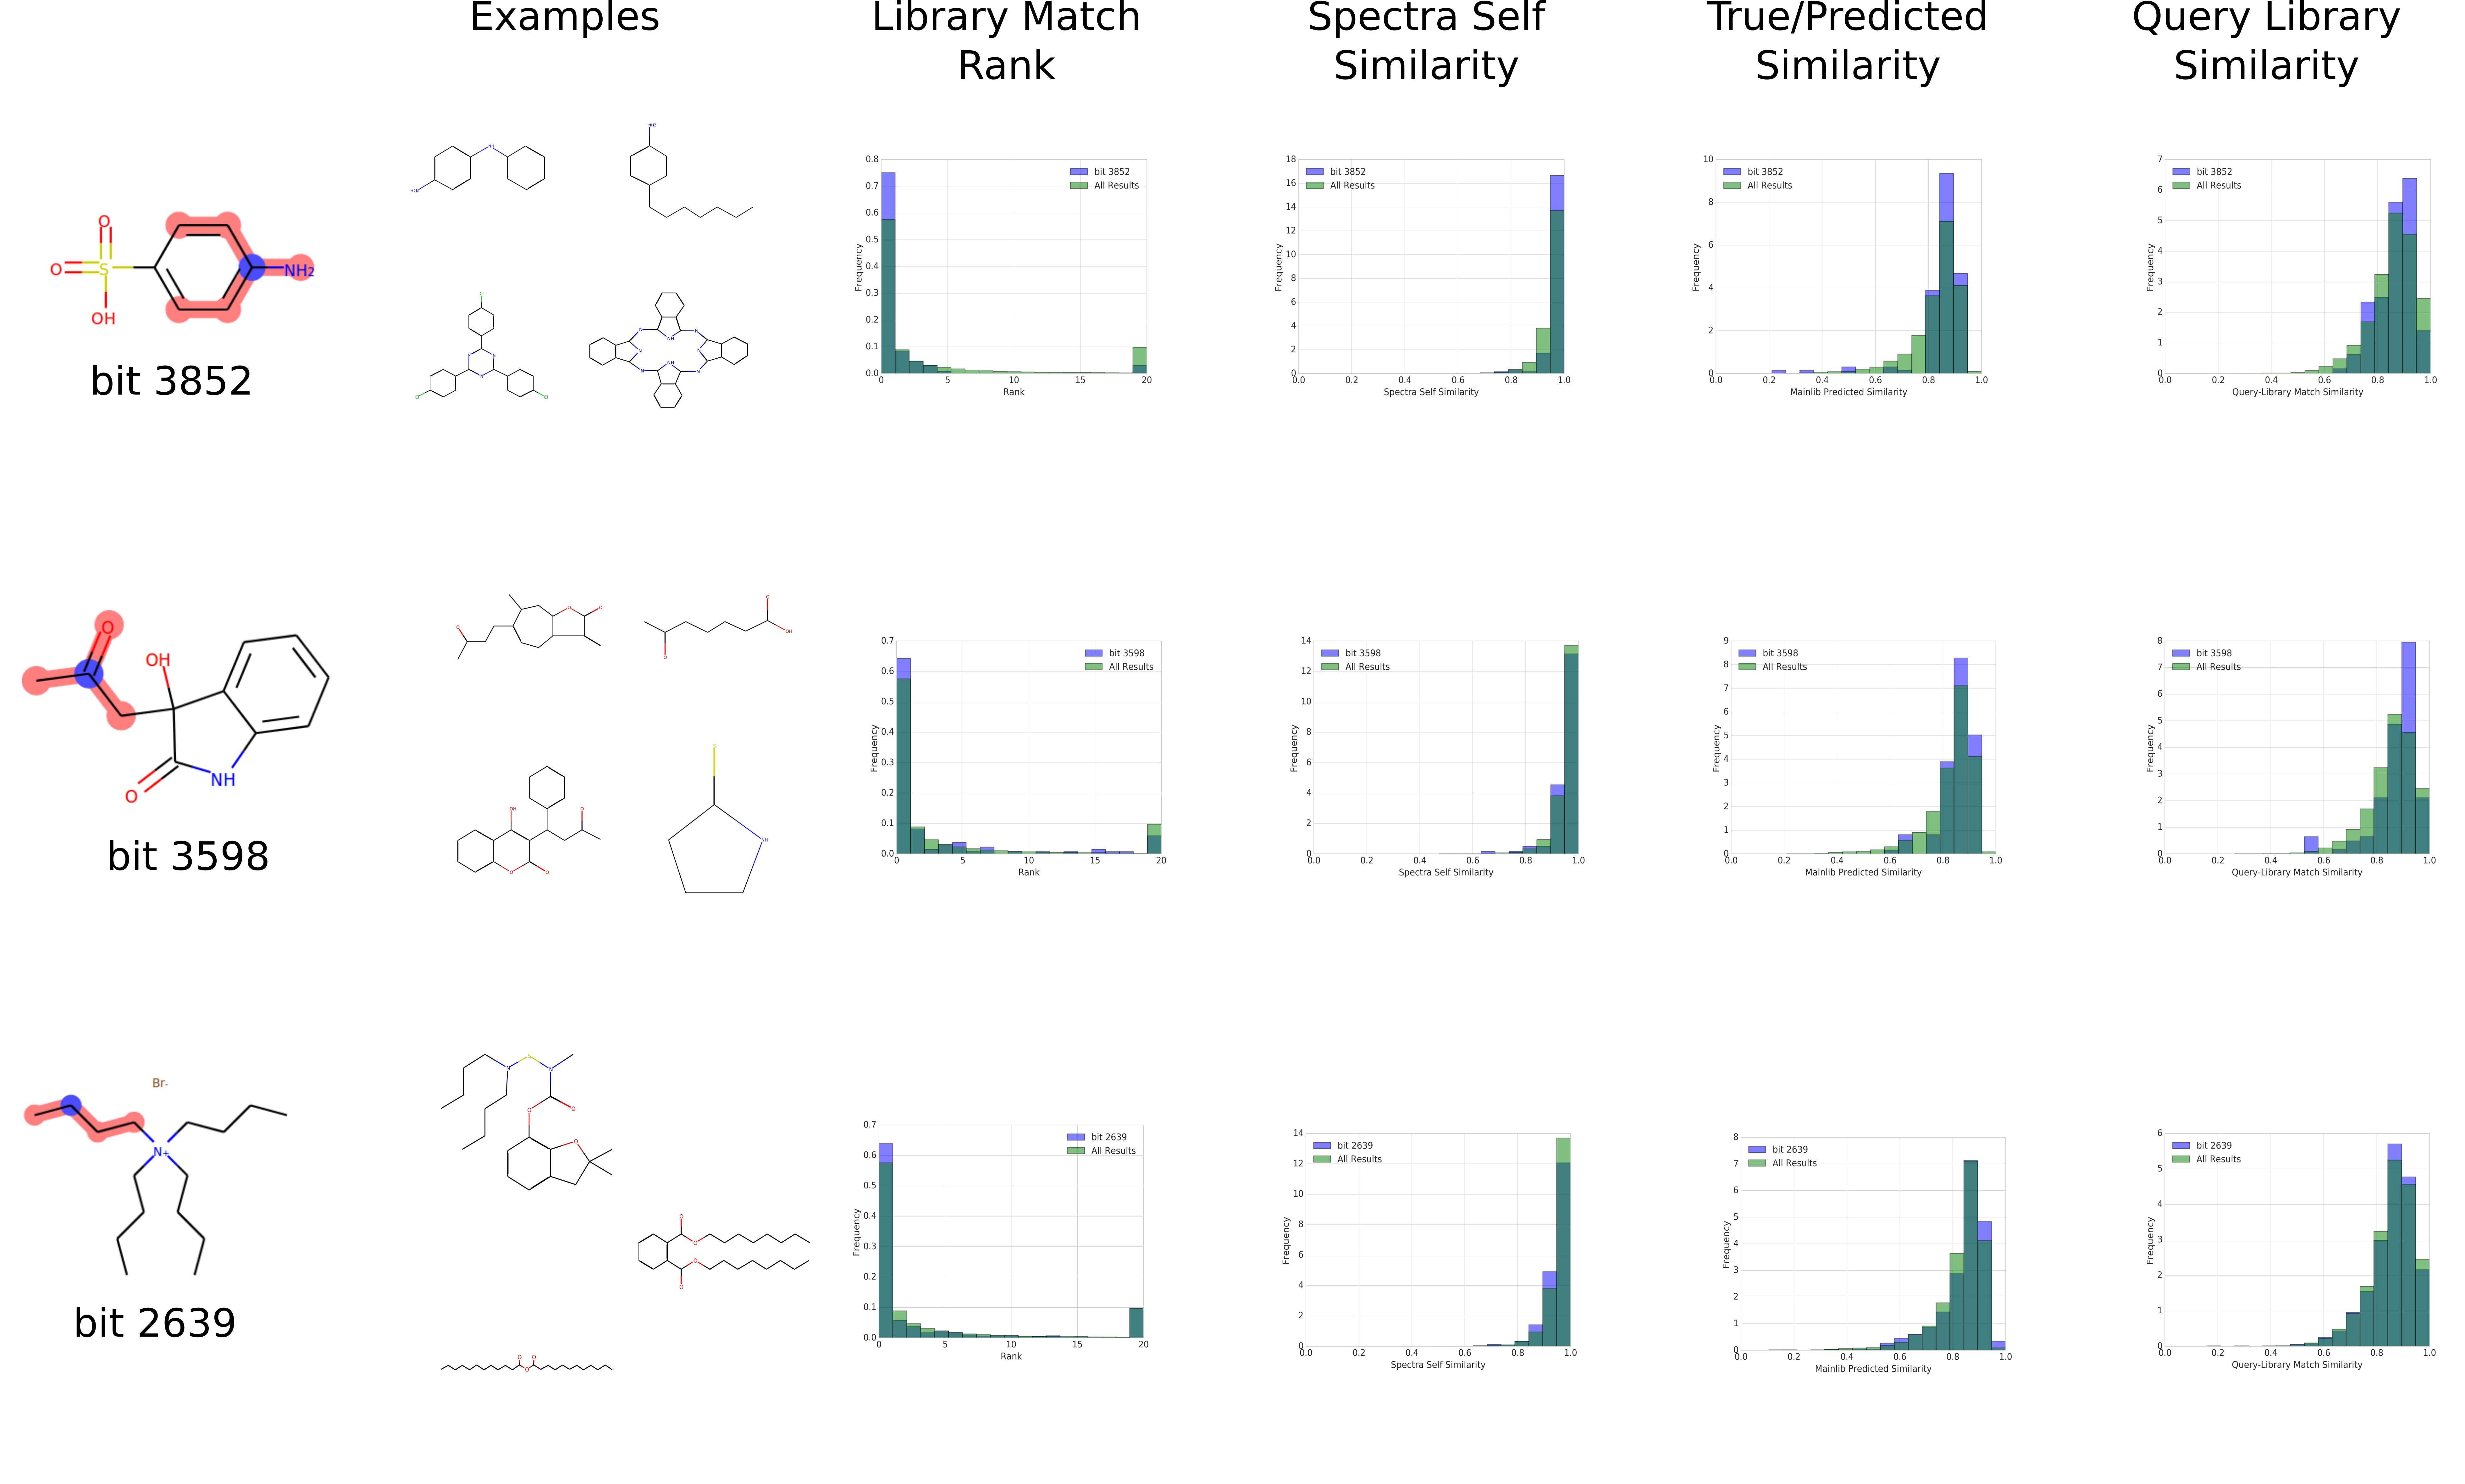
\includegraphics[width=0.95\linewidth]{./figures/bit_analysis.png}
        \caption[Bit Analysis of NEIMS]{Similarities and Library Matching Ranks for selected bits from NEIMS. In blue, we have the distribution for molecules in the query set containing the specified bit, in green, we have the distribution for molecules in the entire query set. The first spectral column, Library Match Rank, is the distribution of ranks received by the predicted spectrum for the given molecule. The second column, Spectra Self Similarity is the noise inherent in the NIST dataset for molecules of these spectra. True/Predicted Similarity refers to the similarity between the predicted spectrum from NEIMS and ground truth spectrum from the main library. Query Library Similarity refers to the similarity between the query spectrum and the library matched spectrum.}
    \label{fig:bit_analysis}
\end{figure}


\begin{figure}[h]
    \centering
    \begin{subfigure}[b]{0.48\linewidth}
        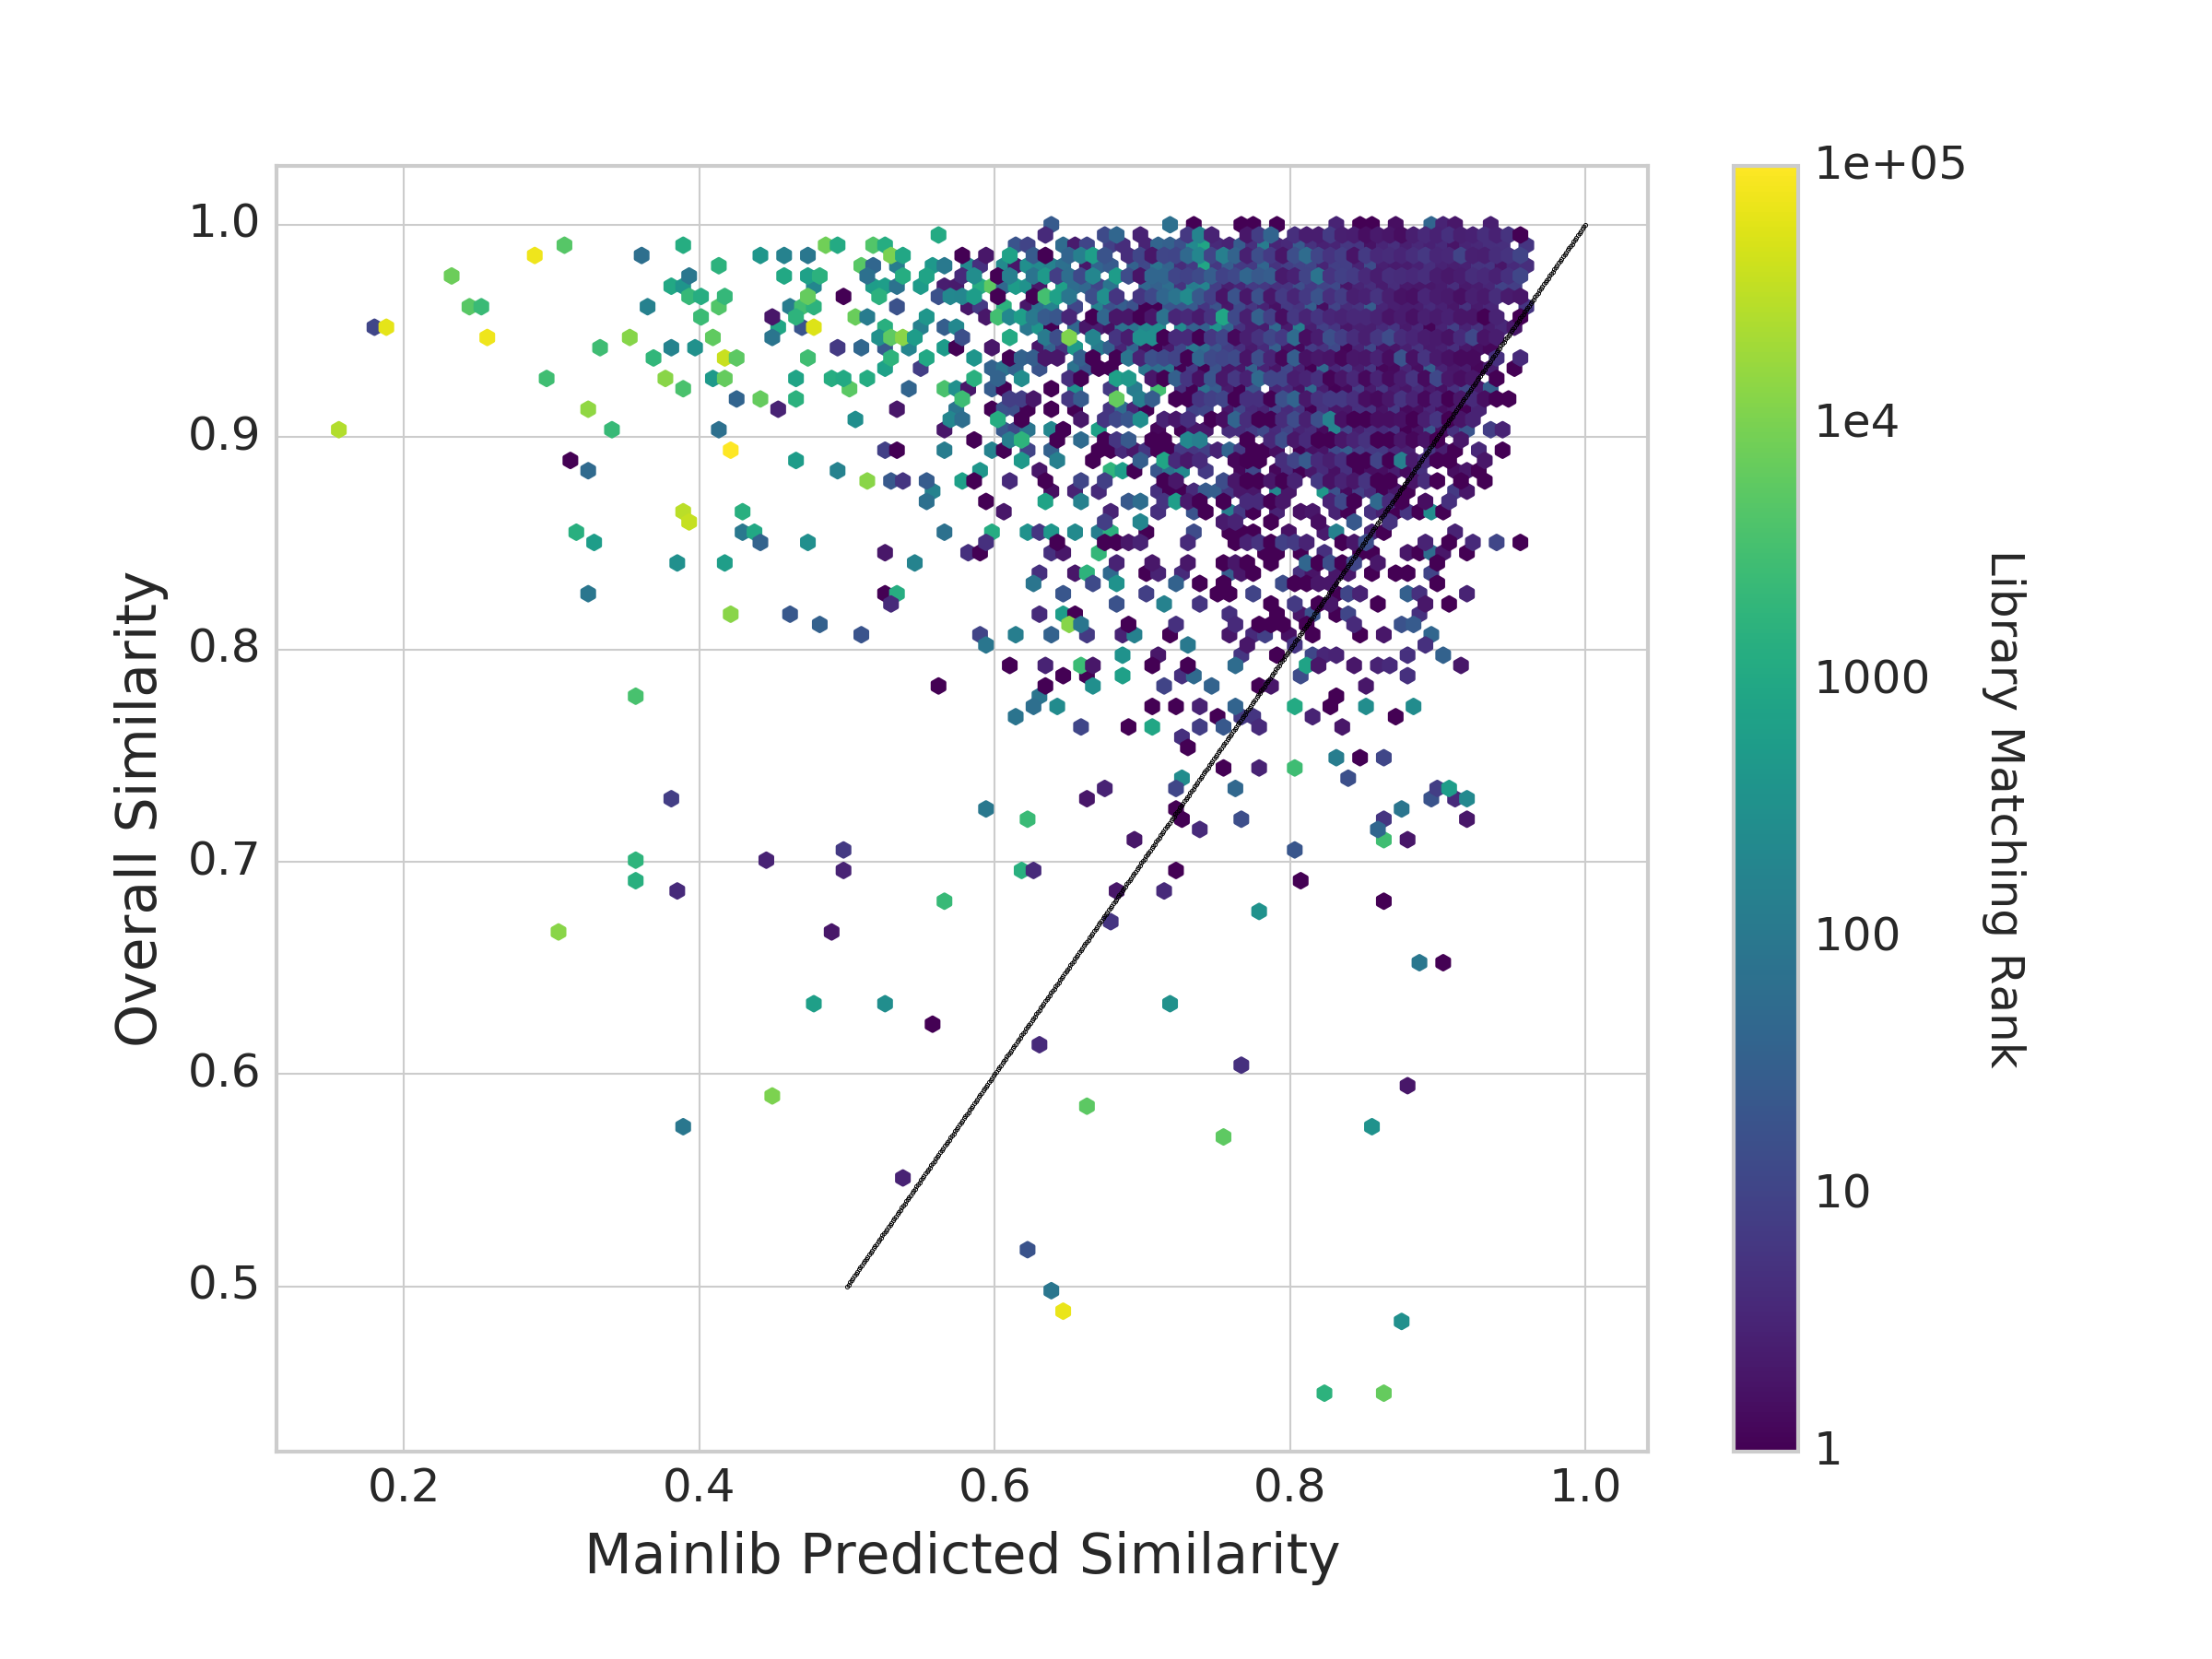
\includegraphics[width=\linewidth]{./figures/Similarity_plot_overall.png}
        \caption{}
        %\caption{Spectral Prediction Similarity vs. Spectral Self Similarity}
    \end{subfigure}
    \begin{subfigure}[b]{0.48\linewidth}
        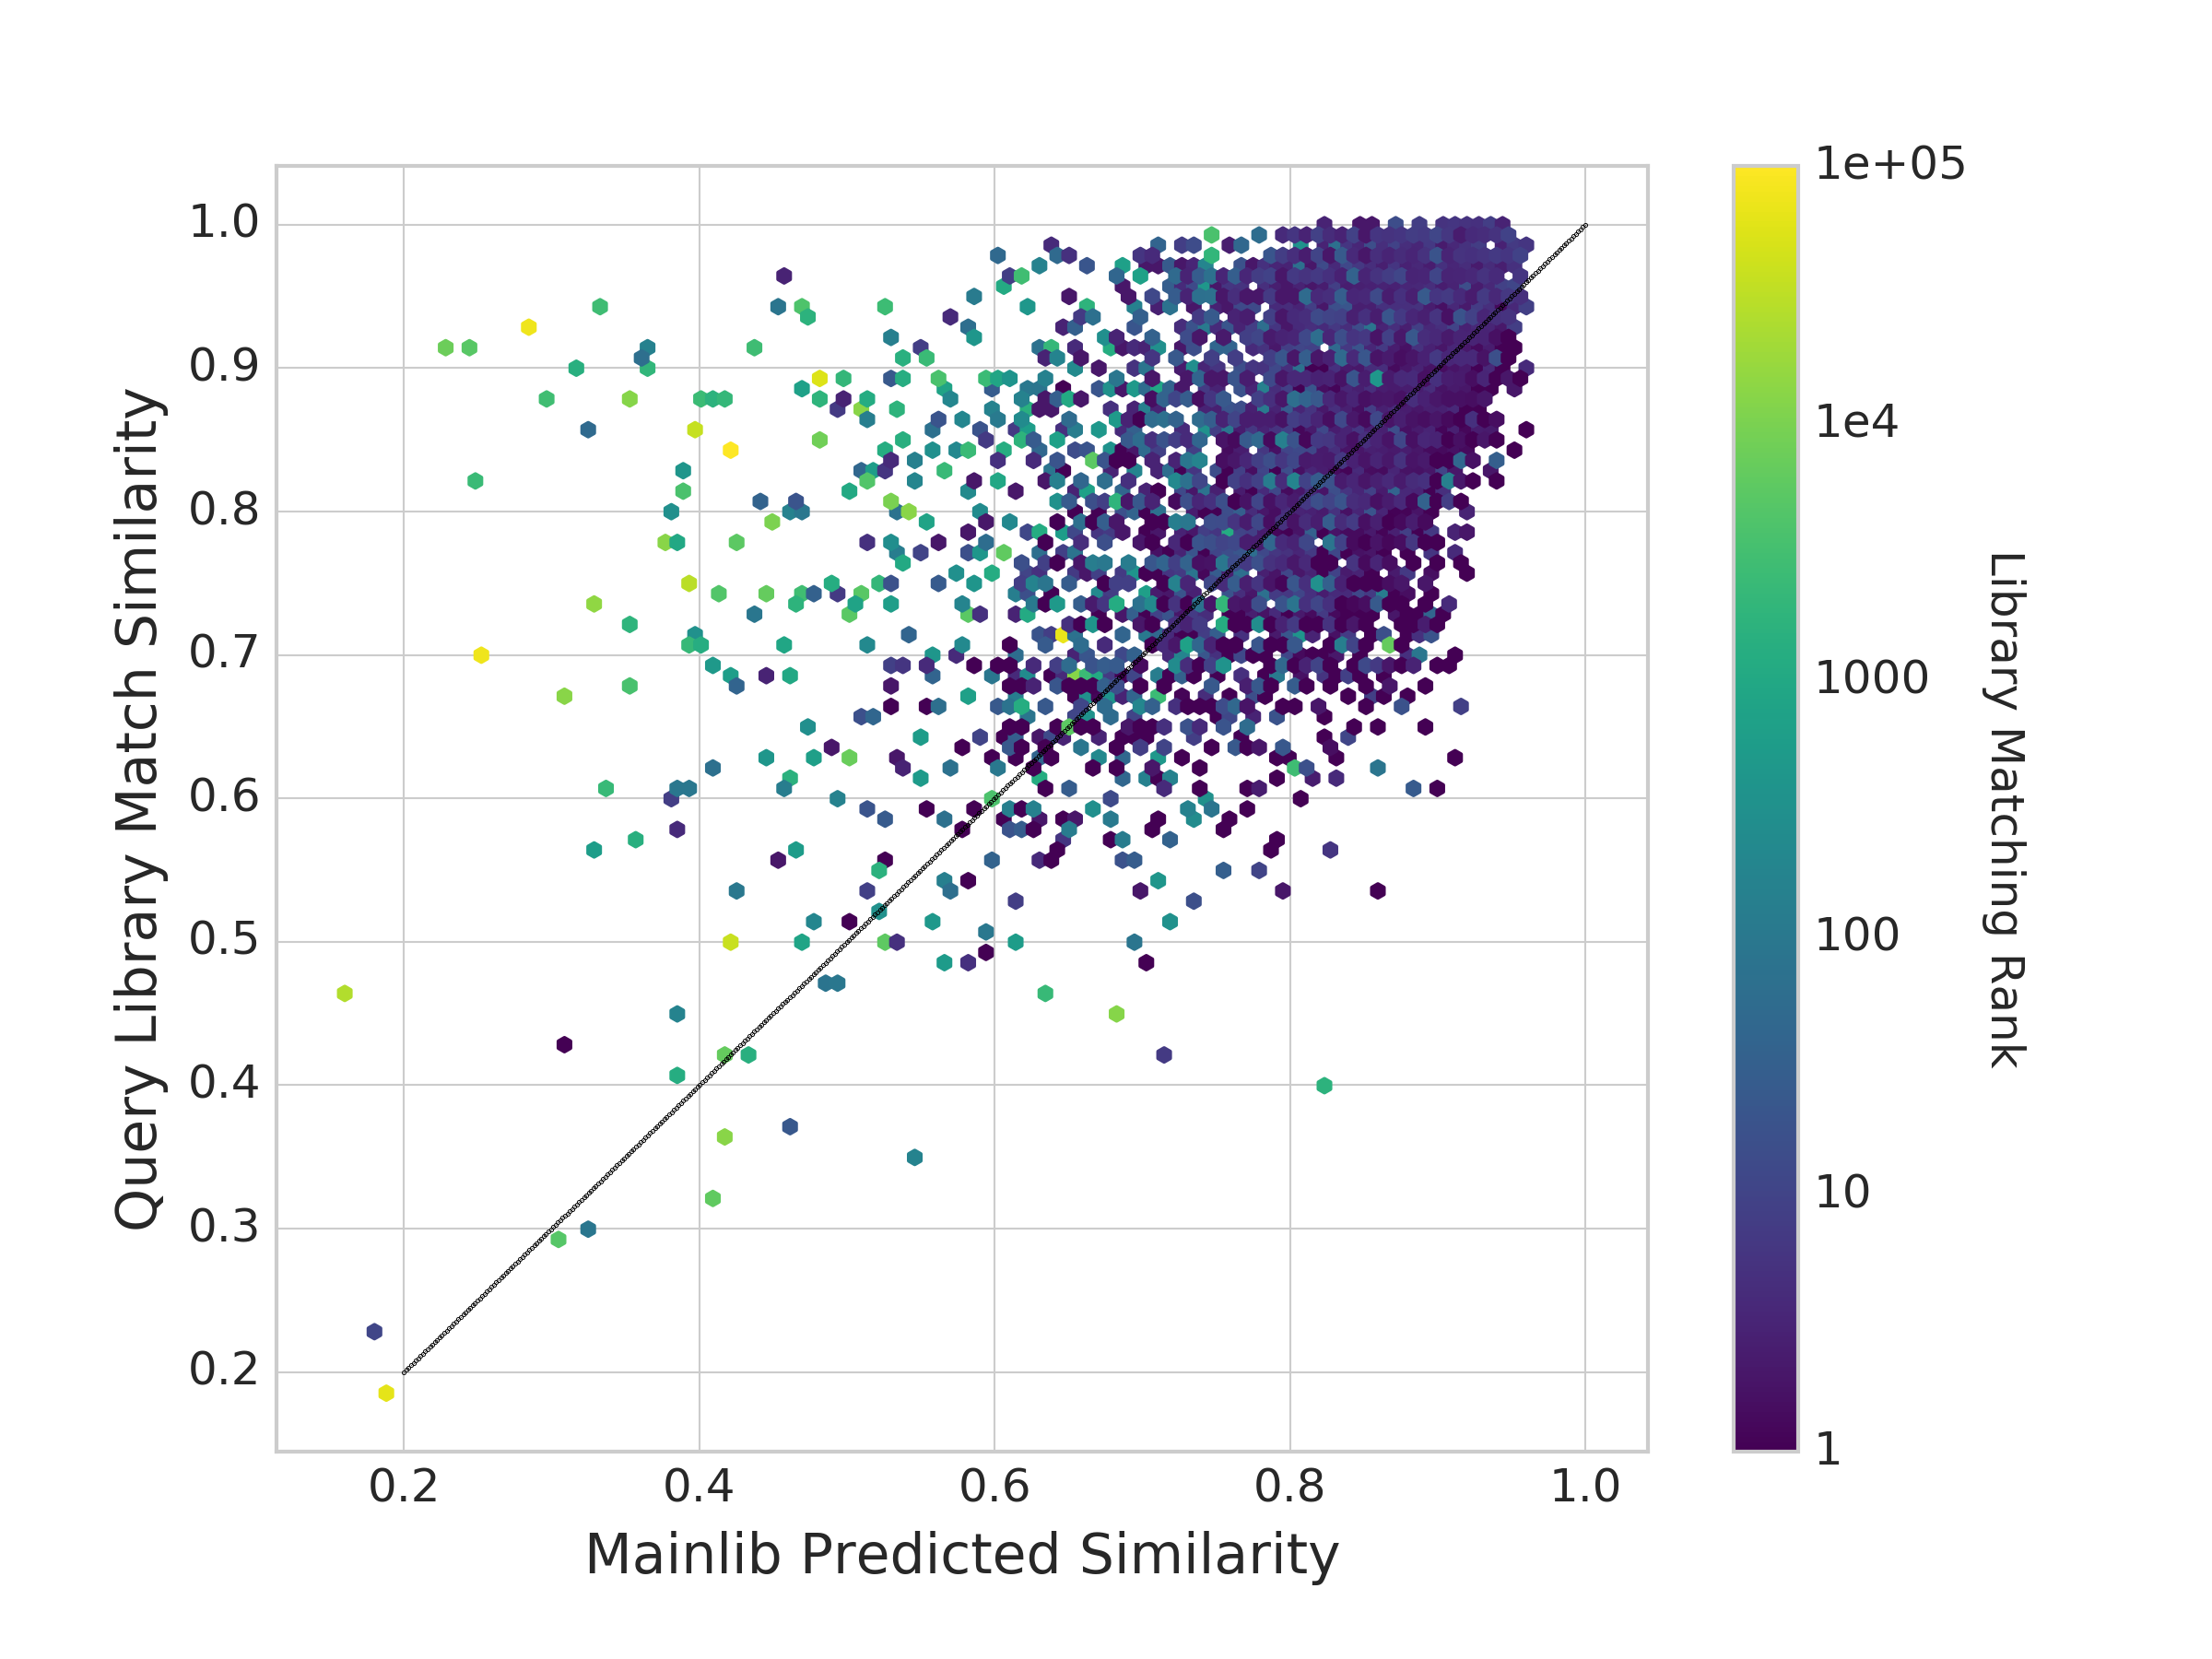
\includegraphics[width=\linewidth]{./figures/similarity_plot_library_match.png}
        \caption{}
        %\caption{Spectral Prediction Similarity vs. Query Libray Matched Spectra Similarity}
    \end{subfigure}
    \caption[Similarity Measurements for Spectral Predictions]{Similarity comparisons for spectral predictions. Color indicates library matching rank of true spectra, with 1 being the best rank. In both figures, the predicted/ground truth spectral similarity is the x-axis. Figure a) compares the predicted similarity against the Overall similarity, i.e. the similarity between spectra in the NIST mass spectral librarie. Figure b) compares this value against the library matching similarity.}
    \label{fig:similarity_scatter_plots}
\end{figure}